\section{Preliminaries}

\subsection{Concepts}
\begin{figure}[t!]
\centering
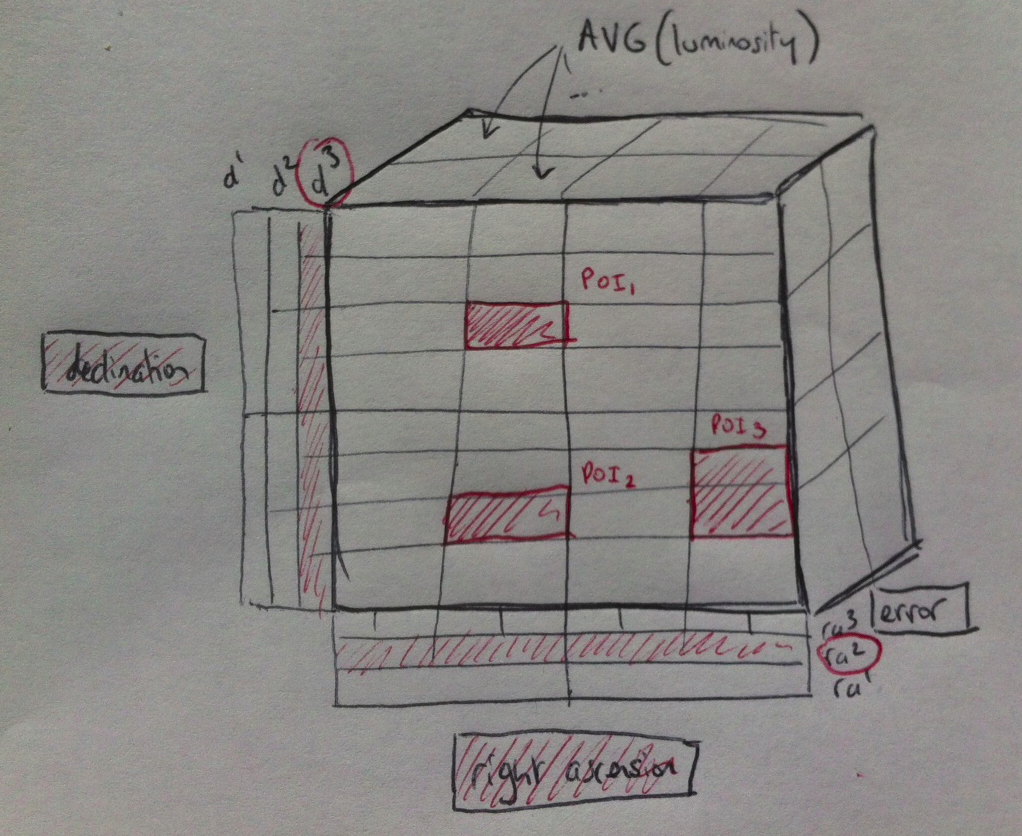
\includegraphics[width=0.9\columnwidth]{images/cube}
\caption{Example of recommendation}
\label{cube}
\end{figure}
We model the database as a large relation $DB$. This table contains two types
of columns: the dimensions $D_0, \ldots, D_d$ and a target column $T$. The
target column contains the target value for each tuple. Note that this view is
logical: we are oblivious to the physical structure of the data.  Claude's aim
is to generate a set of \textbf{explanations}.  An explanation contains two
elements: a \textbf{view} and several \textbf{points of interest} (POI). A view
is an ``informative'' set of dimensions, on which we project the data.  A point of
interest is a selection over this view. It contains tuples for which the target
has a ``remarkable'' distribution.

We illustrate these concepts with Figure \ref{cube}. Our example database
describes light sources.  It contains three dimensions: \texttt{right
ascension}, \texttt{declination} and \texttt{error}. The first two describe a
source's position. The third one describes the measurement errors. For each
tuple, we target the value of the column \texttt{brightness}. Claude's output
is highlighted in red. It contains a view based on \texttt{right ascension},
and \texttt{declination}. We see that the view is a SQL query with the
following structure:
\begin{verbatim}
SELECT   D1, ... , Dn , AVG(T)
FROM     DB 
GROUPBY  D1, ... , Dn
\end{verbatim}
The $n$ distinct variables $\texttt{D1} \ldots \texttt{Dn}$ define the view. Once
Claude has chosen a view, it must explain \emph{why} it has chosen this view.
This is the role of POIs. In Figure \ref{cube}, Claude suggests four POIs. We
can express them in SQL as follows:
\begin{verbatim}
SELECT   AVG(T)
FROM     DB
WHERE    D1 BETWEEN l1 AND h1
 AND     ...
 AND     Dn BETWEEN ln AND ln
\end{verbatim}
The POIs are defined by the ranges $\texttt{[l1,h1]}, \dots \texttt{[ln,hn]}$.


\subsection{Informative explanations}
\label{sec:infor}
\begin{figure}[t!]
\centering
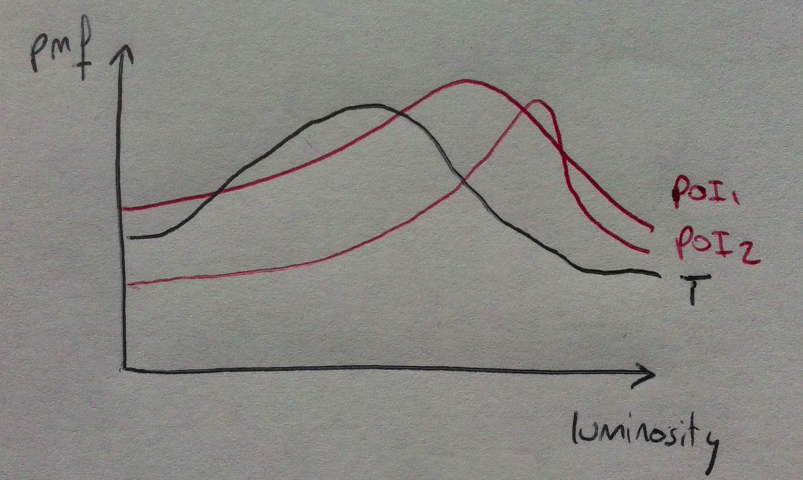
\includegraphics[width=\columnwidth]{images/poi}
\caption{The POIs have unusual distributions}
\label{poi}
\end{figure}

We defined Claude's search space: we want to suggest views and POIs. We now
present how the target helps us recognize the ``interesting'' ones. 

First let's explain how to choose the views. A set of columns is informative if
it is somehow related to the target: if we filter the data on these columns, the target
value changes.  We model this relationship with statistical dependency. We
represent each  dimension $D_k$ by a random variable $\rv{D}_k$. We model the
target with a random variable $\rv{T}$.  A view is interesting if there exists
some statistical dependency between its columns and the target. We formalize
this statement with Mutual Information \cite{cover2012elements}:

\begin{definition}
Consider a view $V = \{D_1, \ldots, D_n\}$, and the target column $T$.  Let
$I$ denote the \emph{Mutual Information} between two random variables. We
define the \textbf{strength} of $V$ as follows:
\[\sigma(V) = I(\rv{D}_1, \ldots, \rv{D}_n ; \rv{T})\]
\end{definition}

Claude seeks variables which are jointly related to the target. Note that it
considers any kind of statistical relationship, not only correlation.
The next step is to extract the POIs. The POIs contain tuples for which the
measure have an ``unusual'' distribution compared to the rest of the database.
Consider Figure \ref{poi}. The curves show the probability mass function of the
brightness for three sets of tuples: the whole database, $POI_1$ and $POI_2$.
The sets $POI_1$ and $POI_2$ come from the view \texttt{right ascension -
declination} in Figure \ref{cube}. We observe that they deviate from $DB$.
They illustrate how right ascension and declination can influence
brightness. We quantify this observation with the Kullback-Leibler
divergence:

\begin{definition}
Consider a range $R = [l_1, h_1] \times \ldots \times [l_n, h_n]$. 
The random variable $\rv{T}_R$ describes the target for
the tuples in $R$, and $\Pr(\rv{T}_R)$ its distribution.
We define the \textbf{divergence} of the range $R$ as follows: 
\[\delta(R) = KL \big( \Pr(\rv{T}_R) \| \Pr(\rv{T})  \big)\]
\end{definition}

The Kullback-Leibler divergence measures the difference between two probability
distributions. Our function $\delta$ grows when a range has unsual target
values, it decreases otherwise. It does not target specifically high or low
values. It seeks \emph{any} type of deviation from the target's global distribution.
Note that divergence is tightly related to strength:

\begin{lemma}
Let $V$ denote a view. We discretize each variable. The variable $\rv{R}$
describes a random bin.  We observe the following relationship:
\[
    \sigma(V) = \mathbb{E}_{\rv{R}} \{ \delta(\rv{R}) \}
\]
\end{lemma}

\begin{proof}
Let $\rv{V}$ represent the joint distribution $\rv{D}_1, \ldots, \rv{D}_n$.
We have $\sigma(V) = I(\rv{V},\rv{T})$.
By definition of the Kullback-Leibler divergence, we have: 
$I(\rv{V},\rv{T}) = $ $\mathbb{E}_{\rv{V}} \{ KL( \Pr(\rv{T} | \rv{V}) \|$ $ \Pr(\rv{T}) ) \}$
As the data is discretized, $\rv{V}$ and $\rv{R}$ are equivalent. Also,
for any bin $R$, $\Pr(\rv{T} | \rv{V} = R)$ is equivalent to
$\Pr(\rv{T}_R)$. We derive the lemma.
\end{proof}


This lemma is simple but powerful. It shows that strength and divergence are
``two sides of the same coin'': the strength of a view equals exactly the
average divergence of its bins. We use the terms strength and
deviation interchangeably to characterize an \emph{explanation} (recall that a
explanation contains both the view and its POIs).

\begin{definition}
Let $S=(\{ D_1, \ldots, D_n\}, \{R_1, \ldots, R_r\})$ describe an explanation . The
\textbf{strength} (or \textbf{divergence}) of $S$ equals the strength
of its view.
\end{definition}

We are now ready to formulate our problem.

\begin{problem}
Consider a hypercube $DB$, a target column $T$ and a triplet $(q, n, r)$. Find
the top $q$ strongest explanations, with $n$ variables and $r$ POIs.
\end{problem}

To solve this problem, Claude operates in two steps. First, it detects $q$
strong sets of columns.  We call this step \emph{column search}.  Then comes
the \emph{POI dectection} step: for each view we extract $r$ POIs. In practice,
our top $q$ strategy can generate redundancy. We tackle this problem with an
optional \emph{refinment} step.


\section{Base algorithm}

\subsection{Column Search}
\label{sec:colum}
The aim of this phase is identify the $q$ strongest sets of variables. To begin
with, we introduce an alternative formulation of strength. From here on, we use
the notations $D_i$ and $\rv{D}_i$ interchangeably. We can use the context to
distinguish database columns and random variables.

\begin{lemma}\label{lem:chain}
(Chaine Rule) Consider a view $\{D_1, \ldots, D_i\}$, and a target $T$.
For any column $D_{i+1}$: 
\begin{multline*}
    \sigma(D_1 , \ldots, D_i , D_{i+1}) \\= \sigma(D_1 , \ldots, D_i)
                + I(D_{i+1} ; T | D_1 , \ldots, D_i)
\end{multline*}
\end{lemma}
\begin{proof}
This lemma is a direct consequence of the Mutual Information's chain rule
\cite{cover2012elements}.
\end{proof}

 Lemma \ref{lem:chain} describes how much a view improves if we append a new
dimension. Given a view $\{D_1, \ldots, D_i\}$ and a dimension $D_{i+1}$, it
gives the strength of $\{D_1, \ldots, D_i, D_{i+1}\}$.  For any random
variables $X,Y,Z$, the notation $I(X;Y|Z)$ expresses the \emph{conditional
mutual information}. It describes the dependency between $X$ and $Y$,
\emph{given $Z$}. The influence of $Z$ can go either way: it can weaken or
strengthen the relationship between $X$ and $Y$. This value is always positive
or null \cite{cover2012elements}.  According to the lemma, the contribution of
$D_{i+1}$ equals the Mutual Information between $D_{i+1}$, and the target given
the view's variables. 

From this observation, we can build a first level-wise algorithm. First, we
enumerate all the sets of exactly one columns. From this set, we obtain all the
sets of two columns. We reiterate until we obtain all the sets of $n$ columns,
and return the $q$ most promising.

Obvioulsy, this procedures does not scale well with the number of dimension
$n$: our algorithm must consider $\sum_{i \leq n} \binom{d}{i}$ candidates,
where $d$ is the number of dimensions in $DB$.  However, $n$ is very small in
practice. It cannot exceed the number of dimensions that a user can visualize
(typically, less than ten).  Also, we can prune the search space:

\begin{lemma}
\label{lem:bounds}
Given a view $V = \{D_0, \ldots , D_i, D_{i+1}, \ldots, D_n\}$:
\begin{align}
    \sigma(V)  & \geq \sigma(D_0, \ldots , D_i) \label{bound1}\\
     \sigma(V) & \leq \sigma(D_0, \ldots , D_i) + H(D_{i+1}, \ldots, D_n) \label{bound2}\\
               & \leq \sigma(D_0, \ldots , D_i) + H(D_{i+1}) + \ldots + H(D_n) \label{bound3}
\end{align}
\end{lemma}

\begin{proof}
Cf. appendix.
\end{proof}

\begin{figure}[t!]
\centering
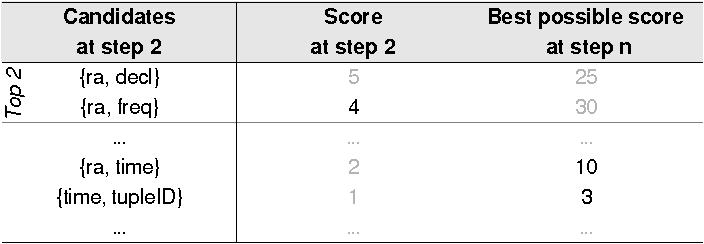
\includegraphics[width=\columnwidth]{images/pruning_example}
\caption{Strength bounds for a few example candidates, i=2 q=2 n=5}
\label{pruning}
\end{figure}

Thanks to these bounds, we can eliminate unpromising candidates.  Consider a
view at step $i$.  Let $\sigma_i$ represent the q\textsuperscript{th} highest
strength obtained so far. If we can predict that our candidate will never
exceed $\sigma_i$, no matter which variables we append to it, then we can
safely discard it. We illustrate this
strategy with Figure \ref{pruning}. The table displays four candidates, for
i=2. Consider the set $\{time, tupleID\}$. Any solution based on this set
will have a strength below 3. The second best candidate found so far has
strength $\sigma_2$ = 4. Therefore,we can can discard it.

To calculate the bounds, we can use Equations \ref{bound2} or \ref{bound3}.
Equation \ref{bound2} is the tightest bound, but it is based on the joint
distribution $C_{i+1}, \ldots, C_n$. If $i>n/2$ we do not have to
compute this distribution, we can ``recycle'' it from previous steps of the
algorithm.  Consider the example table.  Suppose that we want a bound on the
strength of the set $\{ra, decl, time, tupleID\}$. We need to compute
$\sigma(\{ra, decl\}) + H(\{time, tupleID\})$. We obtain $\sigma(\{ra, decl\})$
directly from the first candidate. Also, the last line indicates that we
already computed the joint distribution of $\{time, tupleID\}$. We can reuse
the intermediate results to calculate the upper bound. In some cases, we cannot
apply this ``recycling'' strategy. Then, we use the looser bound of
Equation \ref{bound3}.


\subsection{Detecting Points Of Interest}
\label{sec:detec}
During this phase, we find the $r$ most divergent regions for each view.
Fortunatly, this task is an instance of a known Data Mining problem,
\emph{Subgroup Discovery} \cite{klosgen1996explora}\cite{wrobel1997algorithm}.
The aim of Subgroup Discovery is to identify sets for which the target value
maximizes a user-defined quality measure. To solve our problem, we instantiate
the quality measure with the divergence.

In principle, we could use any efficient algorithm from the Subgroup Discovery
litterature.  In practice, we favour the Beam Search heuristic. This algorithm
is simple and widely accepted \cite{van2011non}. It explores the view top-down,
level wise. To run Beam Search, we need two elements: an initial set of
candidates, called the \emph{beam}, and a \emph{refinment operator}. The
refinment operator generatase several specializations for a given candidate. At
each step of the algorithm, we apply the refinment operator to each item in the
beam. We obtain a large set of candidates. We keep the $r$ best ones, and use
them for the next iteration. The operation is repeated until the algorithm
converges, or some minimum cover threshold is met.

In our implementation, we initialize the algorithm with all the tuples in the
view.  To generate the refinments, we use binning.  Consider a set of tuples
from the beam.  We create $b \geq 2$ bins for each column, and return one
candidate per bin. Thus, if the view contains $n$ columns, our refinment
operator generates $n \times b$ candidates for each set in the beam.  In some
Data Warehouses, the dimensions are already organized in a hierarchy (e.g.,
Country > Region > City). Then, we can use the natural aggregates
in the data rather than bins. We start at the highest level, and ``drill down''
as many times as necessary.

As mentioned in the Subgroup Discovery litterature \cite{van2011non}, our
divergence score has a drawback: it favours smaller groups.  Therefore, Beam
Search may converge very late or not at all.  A practical
solution is to alter the model to take the size into account. Let $R$
represents a range with cover $|R|$, and $|V|$ represent the number of tuples
in the view. We use the \emph{weighted} deviation $\delta_w(R) = |R|/|V| \times
\delta(R)$. This new score introduces a penalty for small POIs.

 
\section{Faster column search}

We present two strategies to speed up column search. First, we introduce a
tractable approximation of view strength. Then, we detail a faster search
procedure, based on Beam Search.

\subsection{Approximating the strength of a view}

In Sections \ref{sec:infor} and \ref{sec:colum} we introduce two ways to
compute the strength of a set of variables. Unfortunately, both of them rely on
expensive joint distributions. There is to our knowlege no faster way to
compute the exact value of this score. We propose to use an approximation:
\[
\begin{split}
    \sigma(V \cup \{D_{n+1}\}) & = \sigma(V)   + I(D_{n+1} ; T | D_0, \ldots, D_{n})\\
                           & \approx \sigma(V) + I(D_{n+1} ; T | D_{i})
\text{ for } D_i \in V
\end{split}
\]

The idea behind this approximation is very naive: we assume that $I(D_{n+1} ; T
| D_0, \ldots, D_{n}) \approx I(D_{n+1} ; M | D_{i})$. We ignore the high order
dependencies. In practice, this assumption rarely holds. 
However, this score is easy to compute. Consider
a directed graph in which each vertex represents a variables $D_i$. Each edge
$(D_i, D_{i+1})$ has a a weight $ I(D_{i+1} ; M | D_{i})$.  The obtain the
approximation, we build a spanning tree and sum its weights.

In most cases, we can build several different spanning trees with different
weights. Which one should we use? We introduce two variants.  Our
\emph{pessimistic} approximation $\sigma_- $ uses the weight of the
\emph{minimum} spanning tree.  Our \emph{optimisic} approximation $\sigma_+ $
considers the \emph{maximum} spanning tree. Consider a view $V$ and a variable
$D_{i+1}$. To obtain $\sigma_+(V \cup \{D_{i+1}\})$, we add the lightest weight
between $ D_{i+1}$ and $V$'s variables to $\sigma_+(V)$.  To obtain $\sigma_-(V
\cup \{D_{i+1}\})$, we add the heaviest one.


\subsection{Heuristic Search}
To speed up column search, we enforce a harsher pruning strategy: at each step,
we discard all the views which are not in the top $q$ strongest candidates.
This strategy is equivalent to Beam Search, presented in the context of POI
detection (Section \ref{sec:detec}). It reduces the complexity dramatically:
our algorithm evaluates $\sum_{i < n} q = q \times n$ candidates.  However, it
is a heursitic: it can miss promising regions of the search space.


\section{Eliminating redundancy}
As Claude is based on a top-k approach, its output may be redundant.  The views
may be very similar to each other, and the POIs may be very close.  Some users
prefer small but diverse sets of suggestions. Here again, we exploit the Data
Mining litterature. The ``trick'' is to map Claude's output to an \emph{Itemset
Mining} setting.  The items represent the dimensions, the transactions
represent the views. Our aim is to identify a few ``meaningful'' patterns from
a list of $q$ itemsets. Authors have proposed several ways to tackle this
problem. For instance, the Krimp algorithm is an established paramter-free
strategy, based on the Minimum Description Length principle
\cite{vreeken2011krimp}.


\section{Real-life example: radio astronomy}
The aim here is to showcase Claude with a real life use case: finding
transients in an astronomical database. Here, the database represents several
thousands light sources (e.g., stars). The measure of interest is a statistic,
which describes how much the sources deviate from some physical model. Higher
is better.


\section{Experiments}
